\documentclass{article}
\usepackage[UTF8]{ctex}
\usepackage{geometry}
\usepackage{natbib}
\geometry{left=3.18cm,right=3.18cm,top=2.54cm,bottom=2.54cm}
\usepackage{graphicx}
\pagestyle{plain}	
\usepackage{setspace}
\usepackage{caption2}
\usepackage{datetime} %日期
\renewcommand{\today}{\number\year 年 \number\month 月 \number\day 日}
\renewcommand{\captionlabelfont}{\small}
\renewcommand{\captionfont}{\small}
\begin{document}

\begin{figure}
    \centering
    
\includegraphics[width=8cm]{upc.png}

    \label{figupc}
\end{figure}

	\begin{center}
		\quad \\
		\quad \\
		\heiti \fontsize{45}{17} \quad \quad \quad 
		\vskip 1.5cm
		\heiti \zihao{2} 《计算科学导论》课程总结报告
	\end{center}
	\vskip 2.0cm
		
	\begin{quotation}
% 	\begin{center}
		\doublespacing
		
        \zihao{4}\par\setlength\parindent{7em}
		\quad 

		学生姓名:\underline{\qquad  何为 \qquad \qquad}

		学\hspace{0.61cm} 号:\underline{\qquad 2007020213\qquad}
		
		专业班级:\underline{\qquad 本研(AI)2001 \qquad  }
		
        学\hspace{0.61cm} 院:\underline{计算机科学与技术学院}
% 	\end{center}
		\vskip 2cm
		\centering
		\begin{table}[h]
            \centering 
            \zihao{4}
            \begin{tabular}{|c|c|c|c|c|c|c|}
            % 这里的rl 与表格对应可以看到,姓名是r,右对齐的;学号是l,左对齐的;若想居中,使用c关键字。
                \hline
                课程认识 & 问题思 考 & 格式规范  & IT工具  & Latex附加  & 总分 & 评阅教师 \\
                30\% & 30\% & 20\% & 20\% & 10\% &  &  \\
                \hline
                 & & & & & &\\
                & & & & & &\\
                \hline
            \end{tabular}
        \end{table}
		\vskip 2cm
		\today
	\end{quotation}

\thispagestyle{empty}
\newpage
\setcounter{page}{1}
% 在这之前是封面,在这之后是正文
\section{引言}
计算科学导论与人工智能类:人工智能总结一句话就是未来可期。目前我所了解到有许多的技术在理论上都基本成型,但是可能在现实的运用上,还需要更多的时间去实验,去修正,而等到我们毕业的时候或者往后工作的几年之中,很可能万物皆可智能。对于我个人,得好好把握大学的学习资源和学习时间,提升自己的专业技术与能力,储存实力,在未来里里大展宏图。当然,在课堂上,老师们讲的许多东西实在是太深刻,不是很容易理解,而且面非常的广,但是老师一直强调等专业和基础知识储备足够后再回头阅读这本书,我现在也铭记在心。计算科学导论上学到的还有学习能力,提高判断力,锻炼系统性思维,思考怎样快速成长等。

\section{对计算科学导论这门课程的认识、体会}
\textbf{整体认识:}\par 
计算科学导论所讲授的知识面积大而且深度不浅,我愿意把它理解成我大学学习生活的引子。首先课程让我对计算机有了一定的认识,对计算机学科的定义、概念、历史、发展变化等有了一定的了解;再者课程不仅仅局限课本内容,更是强调一些学习能力的探索与指引,比如老师说的判断力培养,系统性思维锻炼等等,给我带来了不少启发,不仅仅局限于理论,是一些实质性的启发;另外,计算科学导论课程也锻炼了我个人的能力,比如寻找资源的能力,演讲能力,思考能力,判断能力等,这些都是老师在课堂上以及课后任务上潜移默化传授给我的,而且现在能很清晰感受到它的存在。
\par 
\textbf{下面是详细展开:}\par 
\subsection{PPT演讲-锻炼学生能力}
首先,锻炼了我判断能力;从老师所列的一千余课题中寻找自己所感兴趣的一项深入研究,确实需要一定的判断能力,在海量的信息中寻找出对自己课题有用的信息也是对我个人判断力的锻炼。 \par
再者,锻炼了我寻找资源的能力;从高中到大学,我所认识的较大的一个变化即是从跟学到自学,而我觉着自学很需要寻找资源的能力,网上很多垃圾网站,会误导学生思考认识,老师一开始就给我们讲了一些较可信的网站,给我们提供了途径,课程演讲时寻找资源再加以利用是给了我们锻炼,这样一来,真真切切锻炼了我们寻找资源的能力。其实可以说学完计导,我寻找资源的能力是从0到1,从无到有。\par
还有,锻炼了我思考的能力;PPT演讲后老师所提问的问题对我来说很具有针对性,针对了我所未了解的版块,我觉着这又是一种形式来引导我对我所研究的问题加以更深的思考,我觉着老师所考虑到的问题我之所以没考虑到,是我所站的高度太低,所认识的角度也存在问题,这让我认识到自己的问题,更是引导我在思考。\par

\subsection{课堂引导-启发学生}
老师在课堂上给我启发中,我印象最深的三点如下:\par
1,判断力\par
老师课上说,我们学习生活中到处都得判断,我们也需要有一个很强的判断力。这句话对我启发很大,我觉着这句话尤其适合我们大学生活,当然更远的我也看不到,首先去哪个大学,选择什么样的专业,来了大学改确立什么样的大学目标,细化到社团、导师、当不当班委、参加什么活动、什么竞赛、选什么课等等等等,都需要我们去判断,而且这个判断有很大的价值,可能一个小小的决定就会影响一生。\par 
而锻炼提升我的判断力,老师所传授的方法是需要构建自己的知识体系,而知识体系的构建,非一朝蹴成,但离不开一朝一夕的积累,从小的方面开始,不断积累,外加思考,最后需要把各个方面串联起来,构建大的知识框架,知识体系。\par

2,系统性思维\par
很重要的一项能力,也在一定的程度上影响上述的判断力,系统性思维能够影响我的格局观,看待问题的角度,对事物的认识。非常有利于大学乃至人生的学习生活。当然系统性思维和上述的的判断力紧密相连,相辅相成,锻炼系统性思维也需要系统性学习,链式学习,在大学学习思维中要往这方面考虑。\par
3,快速成长\par
快速成长是一项能力,早点掌握这项技能,会更加有利于我日后的成长生活。
如何快速成长,老师说需要的是实践做项目,对此我深有体会,在这第一个学期中,由于班级事务的一些处理上,我发觉我掌握了一些World/Excel的必备技能,而这些技能都是完成任务的过程中所要必备的能力,是我在短期内快速学会的,是时间所逼,你不得不得学会,这也是做项目能快速成长的重要原因,做的过程发现不足,学习去提高能力,还有时间的限制。\par
做项目,做任务的话,在大学,只要主动,总还是有的,就怕你懒,不想,不去做,图舒服,怕挑战,年轻得有年轻的样子,得有发现机遇的眼力,找导员,找导师,找学长,这些机会在大学得好好把握。\par


\textbf{上面提到的个人知识体系建立,我有如下思考:}

就像老师所说的,有的人到了中年,这个知识体系都没能建立起来,有的人则是一辈子都没能建立,我觉着对于这个知识体系的建立,首先得有自己的认识和思考,我个人觉着知识体系的建立无非就是两个字--“学习”,而在刚开始的学习的过程中,我们又无法感受到自己知识体系的存在,不知道这群高楼大厦的地基在哪,基础建设是啥,耀眼的楼顶在哪,所以很难有自己的目的去构建自己知识体系,但是我们能利用学业和兴趣的指引,去着手,去扩展,去构建。\par
把个人的知识体系比作一棵树,专业知识好比树干,兴趣爱好比作树枝,那么这个时候往回看,我们初小学时期学习的知识就应该是树根,而这个树根可以多,可以少,可能对现阶段影响不大,但应该是决定这棵树的上限,而且树根不是任何时候就固定了,是可以改变的;表面的树干体现的是你专业知识的强弱,也是这棵树很重要的一部分,兴趣爱好所表示的树枝算是这可树里比较亮眼的几部分分支,但是绝不是全部的分支,还有其他的分支,而那些其他的分支是等这棵树长出大体轮廓之后发现还不是很nice的时候,觉着有必要要长出来的,这些树枝长出的时候,知识体系这颗大树也有了一定的模样,你能感受到它的存在了,那些树枝就是你有意的添点,来完美这棵树的。\par
这样来看的话,中小学学习的语文,数学,英语,地理,物理,生物,化学,政治等等,这些都是树根,是个人知识体系中的常识,决定上限,但是是时时刻刻可以去学习,可以去补短的;专业知识这个树干能有多粗就要有多粗,没有树干,树不复存在,但是也不能少了兴趣爱好那些树枝,不然就显得很秃,有了兴趣爱好也不能全够,还是很稀,得发现哪里不足,再去点缀,再去主动学习,社会在进步,不足是常态,这样的话,学习也应该是常态,那么这样的话个人知识体系的建立需要的应该是一个终生学习的过程。\par


\section{进一步的思考}

%结合学习的计算科学知识,对分组演讲涉及的问题作进一步的思考。\par

\textbf{对无人机认识和思考:}\par

\subsection{无人机发展历程简介:(文献大部分来源\citep{1})}

无人驾驶飞机简称“无人机”,英文缩写为“UAV”,是利用无线电遥控设备和自备的程序控制装置操纵的不载人飞机,或者由车载计算机完全地或间歇地自主地操作,其研制始于1914年第一次世界大战,在英国的卡德尔和皮切尔两位将军建议下,英国军事航空学会着手研制一种不用人驾驶,用无线电操纵的小型飞机,至此开始了无人机的发展历程。无人机的研制由A.M.洛教授率领一班人马进行研制,其初衷应用于军事,经历了无数的失败,耗时十年,A.M.洛教授最终取得成功。1927年,由A.M.洛教授参与研制的“喉”式单翼无人机在英国海军“堡垒”号军舰上成功地进行了试飞,在当时的世界上曾引起极大的轰动。从严格意义上说,无人机指的是可回收、能遥控操作和自主飞行的无人驾驶飞机,1935年之前的空中飞行器飞不回起飞点,因此也就无法重复使用。蜂王号的发明,使得无人机能够回到起飞点,使得这项技术更具有实际价值。但由于当时科技水平比较低,无人机的性能、可靠性、导航精度、控制能力还达不到实战需要,且在战争中没有发挥明显作用,受军方冷落。20世纪70年代,美国国防部甚至终止了无人机的发展计划。科技在不断发展,无人机的技术也在逐渐成熟,直至1982年以色列首创无人机与有人机协同作战,无人机才重回大家的视线。20世纪90年代末,美国军方认为无人机的发展对于美国军方的战术空中力量将产生巨大帮助,所以在科索沃战争中美国军方看到了无人机技术的缺陷后财政拨款支持无人机研发事业。21世纪初,由于原来的无人机个头较大,目标明显且不易于携带,所以研制出了迷你无人机,机型更加小巧、性能更加稳定,一个背包就可搞定。同时无人机更加优秀的技能,催发了民用无人机的诞生。2006年,影响世界民用无人机格局的大疆创新无人机公司成立,经历十余年的改革创新,大疆创新公司飞速发展,成为了无人机领域的独角兽,同时也促使了无人机在多个领域的发展应用。\par


\subsection{中国无人机现状总分析:\citep{2}}

我国无人机领域发展十分迅猛,无人机市场这几年的爆炸式增长,特别是民用无人机,已然发展为全球性的优势产业,有很多小伙伴会觉得无人机的市场到头了,其实并不是。随着2019年人社部,发布关于认定13个新职业之中,无人机也在其中,再看看今年人社部发布包括“无人机装调检修工”在内的16个新职业,再次提到关于无人机。从另一方面看,现在很多小学、初中都有开展无人机科普,中高职院校、大学都已开设无人机这方面的专业,未来,随着国家政策逐步落地,市场发展愈发成熟,我国无人机产业或将迎来新一轮爆发。所以我觉着无人机这个市场仍有很大的发展前景。\par

其实,严格意义上来说饱和的是消费级无人机这一块,笼统的说就是我们平常所说的航拍无人机。无人机已经渗透到人们生活的各个领域,影视拍摄、地质测绘、灾情勘察、农业植保……随着人工智能技术的逐步完善,智能硬件开始向小型化、低成本、低功耗方向迈进,这同时也加快了无人机向“集约化”发展的进化历程,行业应用工业级无人机才是未来发展的重头!\par

\subsection{无人机应用领域:\citep{8}\citep{7}}

现代无人机经过数十年的发展,已经应用于农业植保、农药喷洒、电力巡视、交通管制、物流配送、灾后救援、娱乐消费、工程测绘、环境监测、通信连接、警用管制、安防监控、军事反恐等众多领域,在部分领域扮演着不可或缺的角色。\par

\par
\begin{figure}[h!]
\centering
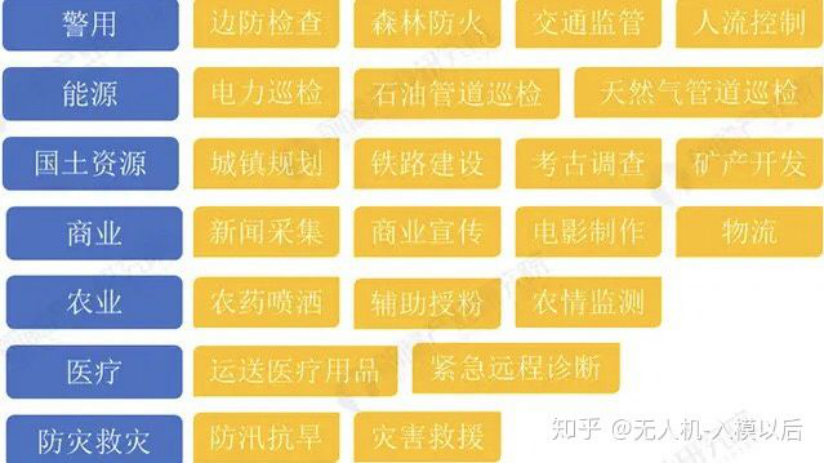
\includegraphics[scale=0.5]{1}
\caption{无人机应用领域}
\label{fig:1}
\end{figure}







\subsection{中国无人机领头公司:}
1.大疆创新\par
深圳市大疆创新科技有限公司,2006年由香港科技大学毕业生汪滔等人创立,是全球领先的无人飞行器控制系统及无人机解决方案的研发和生产商,客户遍布全球100多个国家。通过持续的创新,大疆致力于为无人机工业、行业用户以及专业航拍应用提供性能最强、体验最佳的革命性智能飞控产品和解决方案。\par
另外,大疆创新亦有其严格的行业规范,对其无人机产品也有飞行限制等措施保障,我个人觉着大疆创新公司未来的发展前途明朗。\par

\par
\begin{figure}[h!]
\centering
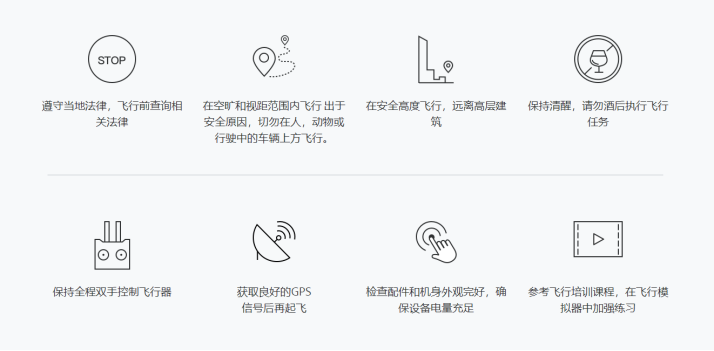
\includegraphics[scale=0.5]{2}
\caption{大疆公司对无人机操作者要求}
\label{fig:2}
\end{figure}








2.亿航\par
广州亿航智能技术有限公司(简称:亿航智能)是一家集研发、生产、销售、服务为一体的智能飞行器高科技创新企业,总部位于中国广州,被著名商业杂志《快公司》评选为2016年全球最佳创新公司。以及全球无人机企业前三强。秉持“让人类像鸟儿一样自由飞翔”的企业使命,亿航智能为各个行业领域客户提供飞行器产品和解决方案,包括自动驾驶飞行器、智慧城市指挥调度中心、行业应用网联无人机、无人机自动化集群编队、无人机物流配送等。\par
\subsection{无人机的特点优势:\citep{4}}

\begin{itemize}

    \item 灵活性:\par
现代无人机体积小,重量轻,拥有飞机卫星无法具备的灵活性;组装之后直接使用,且起飞落地方式简单,对场地要求低,更具有灵活性。\par
    \item 成本:\par
相比较传统飞机,现代无人机的成本相对来说要小很多;\par
而对无人机所应用领域的工作,比如勘探、农药喷洒、货物运输等,相比较之前的工作消耗,无人机所消耗的成本也低很多;\par
对操作人员培养成本,无人机对操作人员的培养成本相对传统无人机来说,要低数倍,培养周期半年左右,这也是传统飞机所不能比的。
成本是产业很重要的参考因素,因此这也成为无人机的一个优势。\par
    \item 安全性:\par
首先对无人机本身,隐蔽性好,隐蔽性多应用于军事方面,体积小好,雷达反射面积小,自身生存能力强;\par
其次,在操作人员方面,无人机无人员伤亡风险,相对传统飞机,其安全性大大提高。\par
    \item 续航时间:\par\citep{6}
续航的话,产业顶端的太阳能无人机平均续航时间能够达到十余小时,在军事,勘察,运输等多个领域的应用具有其独特的优势。\par

\end{itemize}

\subsection{当下无人机的发展局限:\citep{3}}\par
现代无人机的发展中存在的局限可以概括如下:\par
\begin{itemize}

    \item 体型与功能的优化问题;\par
    \item 续航时间跟载重能力问题;\par
    \item 自主飞行,自动避障,撞到障碍之后自动恢复平衡能力;\par
    \item 对未知环境自动构建地图,自定位,自导航;\par
    \item 多台无人机的互相协作,自组网技术;\par
上述问题在无人机应用的不同领域中体现。比如对于消费级无人机而言,其续航时间跟载重能力可被接受,不是主要的需求矛盾,而消费级无人机受限于功能,除了航拍很难找出其他需求,因此其对于自主飞行,自定位等方面的需求更大,当然,消费级无人机对信息的传输速度也有一定的要求,而市场上部分无人机在使用特殊通讯设备传递数据的时候可以达到1Gb每秒的传输速度,这比大多数发达国家提供的宽带速度都要快,因此在传输速度方便面,现代无人机已经做的很好了;\par
但是在行业应用无人机领域,续航时间跟载重却成了其发展得主要矛盾,比如快递运输无人机,其续航时间和载重必须保证,另外,自主飞行,自动避障,自定位,自导航这些需求当然也是必须的。\par
另外,无人机还应用很多领域,由于面积太大,无法一一阐述,因此,接下来就将针对性了解上面所讲到的自主飞行,自动避障局限性的现有但为成熟的解决措施。\par


\end{itemize}


\subsection{无人机未来发展的攻坚技术:}
1.非线性模型预测控制(Nonlinear Model Predictive Control ,NMPC)\citep{9}\par
无人机飞行一个最基本的问题是要弄明白怎么从一个地点飞到另一个地点,听起来似乎很简单,但是飞行器的动力学非常复杂,事实上它们总在对付十二维的空间。这个十二位的空间可以转换成一个包括了横轴,纵轴,竖轴和旋转轴的四维空间。在这个四维平面中,计算一个光滑优雅的运动曲线, 然后转换回到复杂的十二维空间来让飞行器获得控制和执行动作。当有多台飞行器协作群体飞行时,每个飞行器还可以监控周围飞行器的距离,来自动调整自身的飞行动作达到分散化的协作效果。其中需要无人机拥有自主飞行,自动避障,撞到障碍之后自动恢复平衡能力,还要有对未知环境自动构建地图,自定位,自导航能力,而提升这些能力,离不开非线性模型预测控制(Nonlinear Model Predictive Control ,NMPC)技术,更具体地说,他们通过NMPC算法来预测无人机周围环境中的障碍物轨迹,同时使用分类模型来区分不同类型的轨迹并预测障碍物的未来位置。\par
比约恩·林德奎斯特是瑞典吕勒奥工业大学和加利福尼亚理工学院联合研究团队中的一员,近日,该团队在IEEE Robotics and Automation Letters上发表的一篇最新论文\par

\par
\begin{figure}[h!]
\centering
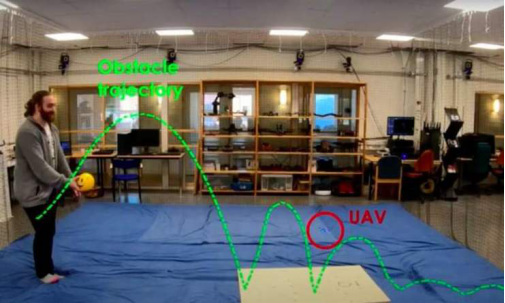
\includegraphics[scale=0.3]{3}
\label{fig:3}
\end{figure}


研究人员通过四组实验评估了NMPC方案,结果发现无人机模型能够在多个移动障碍物包围的情况下避免碰撞。四项实验分别为:\par

实验一:避免弹球时保持位置:不同方法下,无人机在保持姿势,同时避免任何障碍物方面的性能表现,其中弹球为障碍物。\par
实验二:避开行人时保持位置:无人机在保持姿势,同时避免障碍物方面的性能表现,其中行人为障碍物。\par
实验三:弹跳条件:障碍物提供运动轨迹,检测NMPC对障碍物路径的预测和规避能力。\par
实验四:多重障碍:检测在多种障碍物包围情况下,NMPC系统的规避能力,并测试最小安全距离。\par
实验成果:\par
可预测路径,躲避多个障碍物\par
论文中介绍了NMPC成本函数和约束条件公式化,以及解决动态障碍的方法。同时为了证明所提出的控制体系结构的功效,也进行了多种情况下的测试实验。\par
实验一:避开弹丸时保持位置:无人机的任务是避开任何进入的障碍物而保持飞行姿势,其中障碍物是向无人机发射弹球。论文中,NMPC约束方法与人工势场等其他方法进行了比较(静态环境下能够快速响应并躲避障碍物)。\par
考虑到障碍物的静态性,空间半径和障碍物半径分别设置为1m,这比避免静态障碍物所需的安全距离要大得多,同时将势场控制器的参考调整为尽可能积极。放宽NMPC的输入速率约束,以加快响应速度。\par

\par
\begin{figure}[h!]
\centering
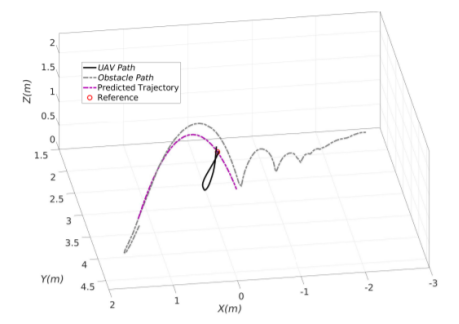
\includegraphics[scale=0.5]{4}
\label{fig:4}
\end{figure}


在保持与缓慢移动的障碍物的距离的同时,这两种方法都无法避免与弹丸障碍物发生碰撞,障碍物进入影响区域的时间很短, 这些控制器直到与无人机发生碰撞,才能及时避开,而且这些控制器也不知道障碍物的未来位置在哪里,因此,它们的避让动作可能会使它们沿着障碍物的轨迹移动。\par
实验二:避免行人时保持姿势:实验中,“行人”在直接碰撞过程中向无人机走去,以测试无人机的避障能力和反应速度。\par

其中,行人在0.3 s内进入实验障,碍物的半径设置为0.6 m,从无人机和障碍物的路径可以看出,从识别出轨迹的时间步长开始,飞行控制器便开启了回避机制。\par
实验三:与前两种情况一样,无人机的任务是保持位置,同时避免进入的障碍物。障碍物半径设置为0.4m,被抛出经过第一次反弹后影响无人机路径。\par
如图,投掷障碍物的时间约为0.25 s,而控制器的反应速度为0.35 s。这表明即使是简化的轨迹模型也仍然可以对障碍物路径做出足够好的预测,尤其是在增加沿预测的安全半径。\par

\par
\begin{figure}[h!]
\centering
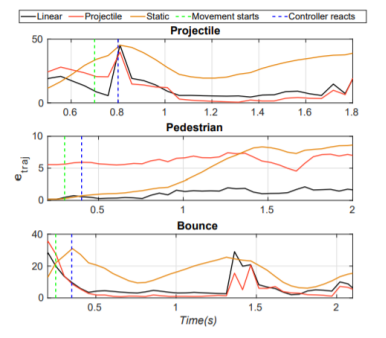
\includegraphics[scale=0.5]{5}
\label{fig:5}
\end{figure}

下图为基于回避操作开始时的初始条件的障碍物的预测轨迹,以及障碍物和UAV的测量路径。\par

\par
\begin{figure}[h!]
\centering
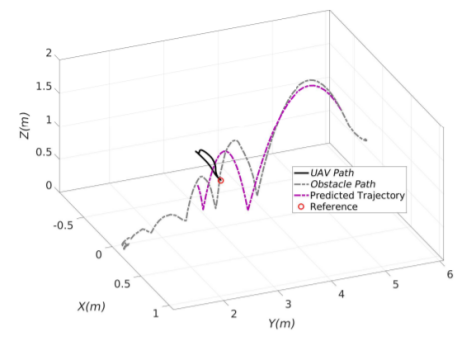
\includegraphics[scale=0.5]{6}
\label{fig:6}
\end{figure}

无人机成功避开了最小距离为0.38 m的障碍物,而求解器时间达到了33 ms的峰值。由于求解器公差和测量结果不理想,因此预期会出现小范围的约束冲突。\par
实验四:避免多个动态障碍,在避开无人机的碰撞航线上设置一架单独的无人机,同时向其投掷弹丸,两者的障碍物半径都设置为 0.4。轨迹分类和预测方案应用于两个障碍物的单独测量,但在其他方面与单个障碍物情况相同。两个无人飞行器和弹丸的轨迹如图,

\par
\begin{figure}[h!]
\centering
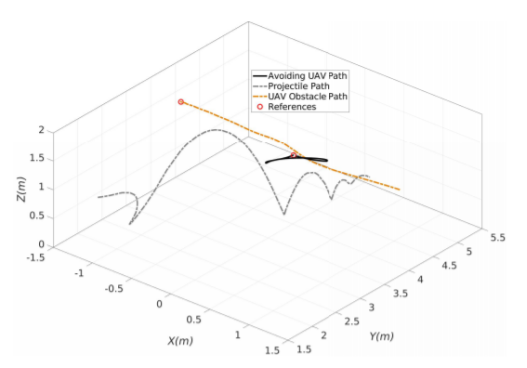
\includegraphics[scale=0.5]{7}
\label{fig:7}
\end{figure}

躲避的无人飞行器、最近的无人飞行器以及障碍物三者之间的最小距离分别为0.45 m和0.42 m。\par

\par
\begin{figure}[h!]
\centering
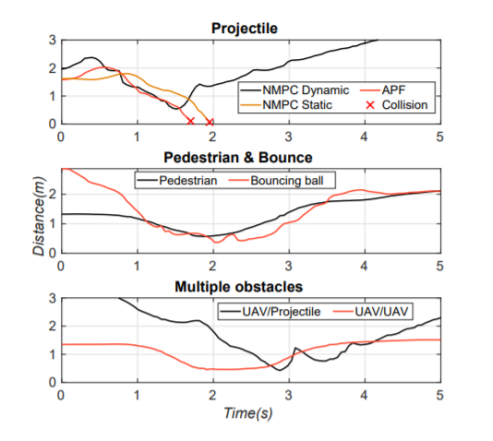
\includegraphics[scale=0.5]{8}
\label{fig:8}
\end{figure}

需要注意的是,避空无人机可以在较长的时间内保持安全距离,同时避开进入的弹丸。实验中,障碍无人飞行器一旦开始运动,回避操纵就会立即开始。\par
进一步研究方向
总体来讲,研究人员所提出的NMPC架构和轨迹分类方案成功地在所有可能的情况下提供了无碰撞运动路径。在线优化问题可以在所需的50 ms的限制内解决,而不会违反已建立的障碍或输入限制。不过,该方法目前也存在一定的局限性:\par

总体性能基于对轨迹分类的依赖:即使对于有限的轨迹研究,其方案也可能出现轨迹分类错误的情况。\par


使用对未来障碍物位置的明确预测:如果预测方案失败或误差太大,无人飞行器可能会完全忽略碰撞过程中的障碍物。\par

论文中指出,未来这项工作还会进一步优化和拓展,具体方向包括更一般的轨迹识别,障碍物位置和速度的提取,轨迹分类方案优化等。更重要的是,随着更多障碍物扩展以及与求解器时间的关系,分析NMPC的复杂性问题,以了解在何时间接地在控制层解决障碍物更合适。雷\par
 
2.自组网技术\citep{5}\par 
无人机自组网的概念:无人机自组网是由无人机担当网络节点组成的具有任意性、临时性和自治性网络拓扑的动态自组织网络系统。作为网络节点,每架无人机都配备移动自组网络通信模块,既具有路由功能,又具有报文转发功能,可以通过无线连接构成任意的网络拓扑。每架无人机在该网络中兼具任务节点和中继节点两种功能:作为任务节点,可在地面控制站或其他无人机的指令控制下执行任务意图;作为中继节点,可根据网络的路由策略和路由表参与路由维护和分组转发工作。\par
无人机自组网系统构成 无人机自组网系统包括一个地面控制站节点和若干个无人机节点。其结构图如图所示,图中1个地面控制站与4架无人机构成1个无人机自组网。在无人机自组网络中,由于无线传输距离限制或地形限制,无人机间的路由有时需要多个网段组成。如图所示,无人机节点C和地面控制站无法直接通信,但可以通过节点D和地面控制站以C→D→地面控制站路由进行通信,或通过节点A、B和地面控制站以C→A→B→地面控制站路由进行通信。\par

\par
\begin{figure}[h!]
\centering
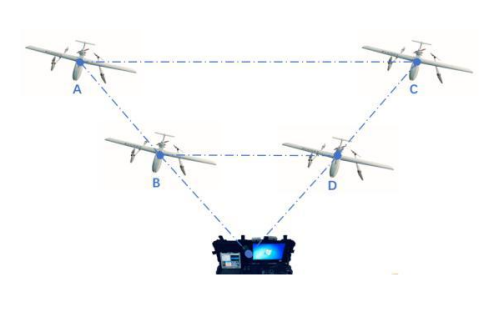
\includegraphics[scale=0.5]{9}
\label{fig:9}
\end{figure}
       
无人机自组网方案特点 无人机自组网除具有独立组网、自组织、动态拓扑、无约束移动、多跳路由等一般自组网网络本身的技术特点以外,还具有以下的任务使用特点。\par
  1.适用于复杂地形、非视距应用 单架无人机容易受到地形或其他环境影响,无法实现无人机和地面的实时通信。但无人机自组网中每个无人机都可作为中继机,可以实现复杂地形下和非视距的应用。\par
  2.适用于远距离作业覆盖由于地球曲率影响,无线电视距传播受到极大的影响,再加上基站周围地形因素的影响,往往通信距离小于50km。当使用无人机自组网通信链路时,离基站最近的无人机除了承担任务机的角色以外,还承担着中继机的角色。当加入中继功能后,数据链的通信距离范围可以增加到150-200km,免去了无人机往返作业及转场的次数,提高了任务效率。\par
  3.抗干扰能力强 自组网网络使所有无人机集群间不再是简单的链式结构,即使在链中的任何环节出现故障,无人机整个系统也不会瘫痪,这就意味着无人机系统的抗干扰能力得到了大幅提高。\par
  4.智能化程度高 无人机自组网能够及时感知网络变化,自动配置或重构网络,保证数据链路的实时连通,具有高度的自治性和自适应能力。另外,无人机自组网可以实现信息共享,能够将所接受的信息进行处理,并自主决策,实现执行任务智能化。\par
  5.功能多样 无人机自组网后就具有所有终端的功能,各无人机优势互补、分工协作,形成有机整体,获得比单机更好的执行任务效果。\par
    6.多路高清数据传输 一次任务可实现多次传统任务效果。任务以无人机环境保护监测为例,由于环境监测面积较大,采用四架无人机同时进行环境保护作业,地面与无人机控制距离达到50km,无人机与无人机最大控制距离达到150km,四架无人机可同时采集FHD视频并实时回传至地面站。若发现环境异常等情况,可派遣多架无人机前往现场上空进行多角度数据采集,同时可避免数据链因地形复杂、山体遮挡造成失联的情况发生。 \par

\par
\begin{figure}[h!]
\centering
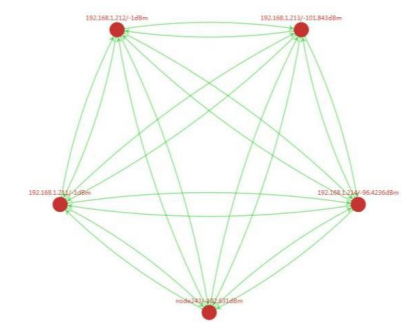
\includegraphics[scale=0.5]{10}
\label{fig:10}
\end{figure}
 
网络拓扑结构
行业应用\par
  1.安防行业应用 防地域范围较大,单架无人机监视范围小,无人机需要多次往返,甚至多次转场才能完全覆盖任务区域,耗时较长、效率低;当无人机出现故障时会影响任务。运用无人机自组网,一次可以完成大面积的监视任务,发现问题时可以使用多架无人机不同角度的去监视;一架无人机出现故障时不会影响执行任务。\par
  2.应急搜救行业应用 在山区人工搜救时,有些地势和环境复杂,单架无人机执行任务时,会出现数据链遮挡影响无人机与地面站的通信的问题。运用无人机自组网,每个无人机都可作为中继机,不会出现数据链遮挡的问题,如图所示。\par
  3.物探行业应用 航空物探需要飞行器长时间进行低空飞行以达到精准的勘探效果,而低空飞行受地球曲率影响无法实现较大的飞行半径。自组网模式则很好地解决了这个问题,通过一架或多架无人机中继桥接,实现了低空长距离勘探。\par
  4. 环保行业应用 环境监测使用无人机自组网,可以根据任务来增减无人机组网数,当环保监测面积较小时可以使用一两架无人机去执行任务;当环保监测面积较大时可以用多架无人机执行任务,可以灵活、高效的完成任务。\par
  \subsection{演讲存在问题思考}
\begin{table}[h]
	\centering
	\caption{问题与思考}
	\begin{tabular}{cl}
		% 这里的rl 与表格对应可以看到,姓名是r,右对齐的;学号是l,左对齐的;若想居中,使用c关键字。
		\hline
		问题 &                      思考 \\
		\hline
		大疆 &1,硬件:锂电池逐步成熟特点轻巧适用于无人机。\\ 
		为何 &2,通信技术:消费级无人机发展需要图片传输,。\\
	    在  &  此时3G兴起,大疆可以说是3G的弄潮儿。\\
        06 &3,中国经济:大疆公司地处深圳,基础工业发达区\\
	    年  &  为其提供了良好的发展环境,而且就近二十年来看,\\
	    以后 &  无人机的飞速发展只可能在中国,因为其他国家的工业已近退化。\\
	    快速 & 4,大疆公司:公司创始人兼董事长汪滔在大学期间跟随\\
		  发展 &的导师研究的是无人机飞行这一块,对其有一定的启发。\\
		\hline
	\end{tabular}
	\label{table1}
\end{table}
  


\section{总结}
%在这里,写自己对于整个课程和或本次报告的总结。\par
课程:\par
课程对我确确实实起到了引子的作用,对我大学生活学习成长,甚至是以后人生的生活学习成长起到了奠基的作用,课程上我学到的东西,对我个人能力的提升要远远高于知识的提升。我对老师所讲深受启发,老师所讲的东西我日后的学习生活一定得好好实践,沉淀。\par
报告:\par
报告无疑是我对课堂知识的一次沉淀,以回顾与总结的方式重新感受本学期所学;另外,本报告加深了我对自身的认识,对我自己是一个很大的帮助;再者说,本报告提升了我写报告的能力。



\section{附录}
\begin{itemize}
    \item 申请Github账户,给出个人网址和个人网站截图
    \begin{figure}[h!]
    	\centering
    	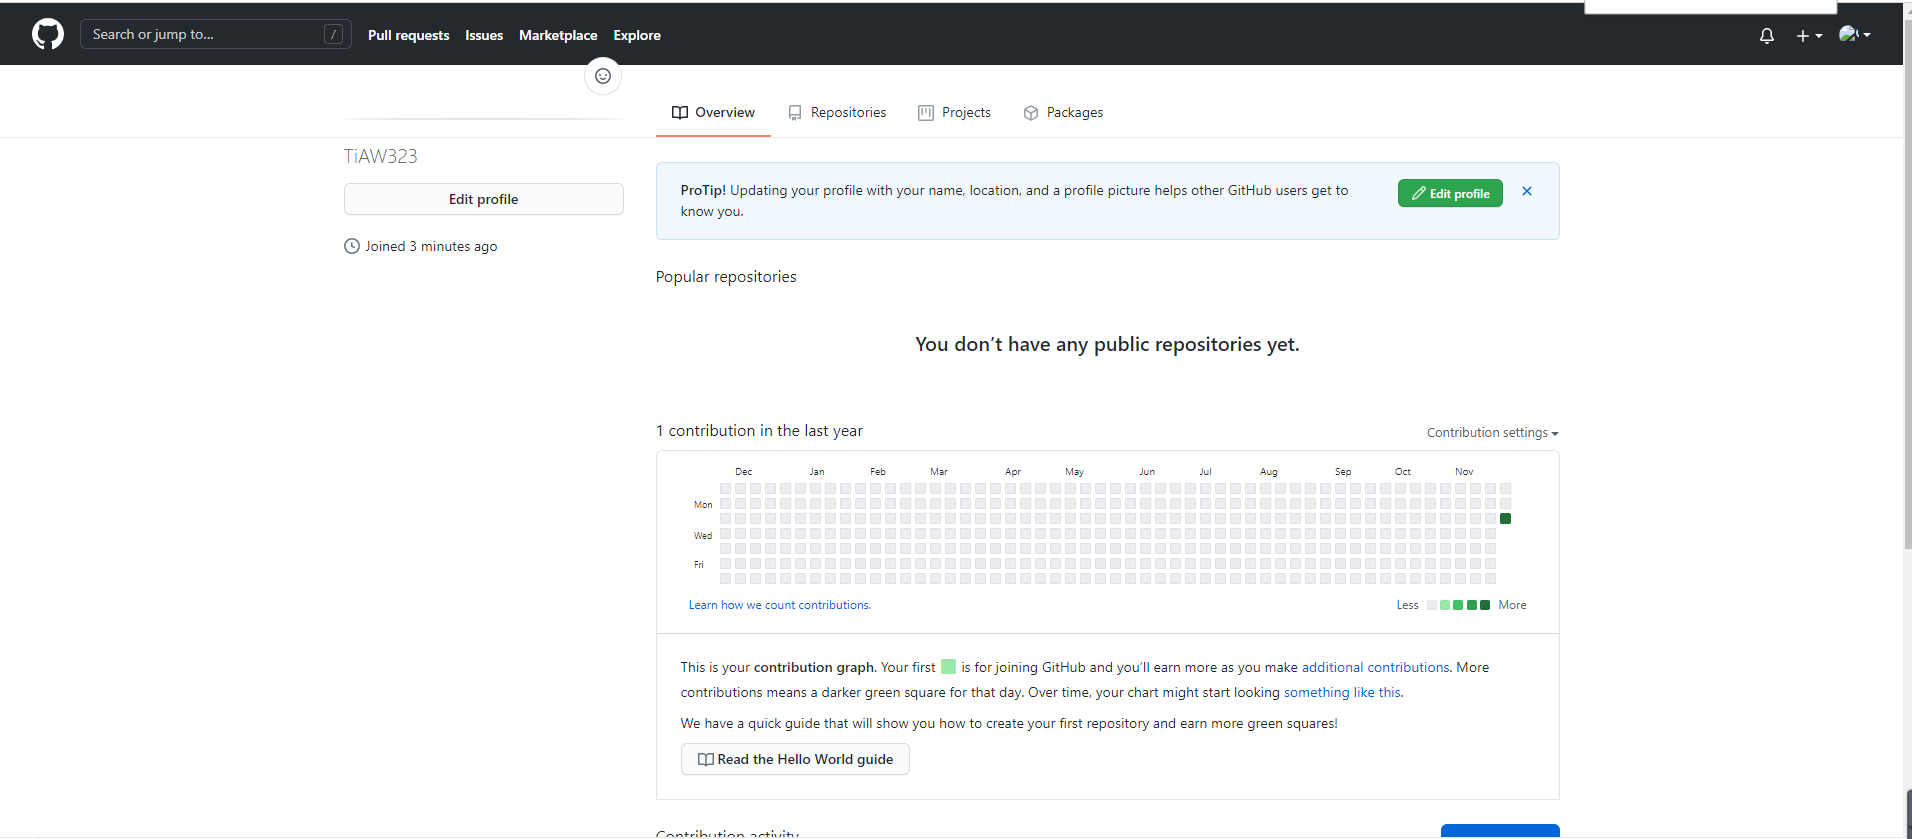
\includegraphics[scale=0.2]{GitHub}
    	\caption{GitHub网址:https://github.com/TiAW323}
    	\label{fig:github}
    \end{figure}
    \item 注册观察者、学习强国、哔哩哔哩APP,给出对应的截图
    \begin{figure}[h!]
    	\centering
    	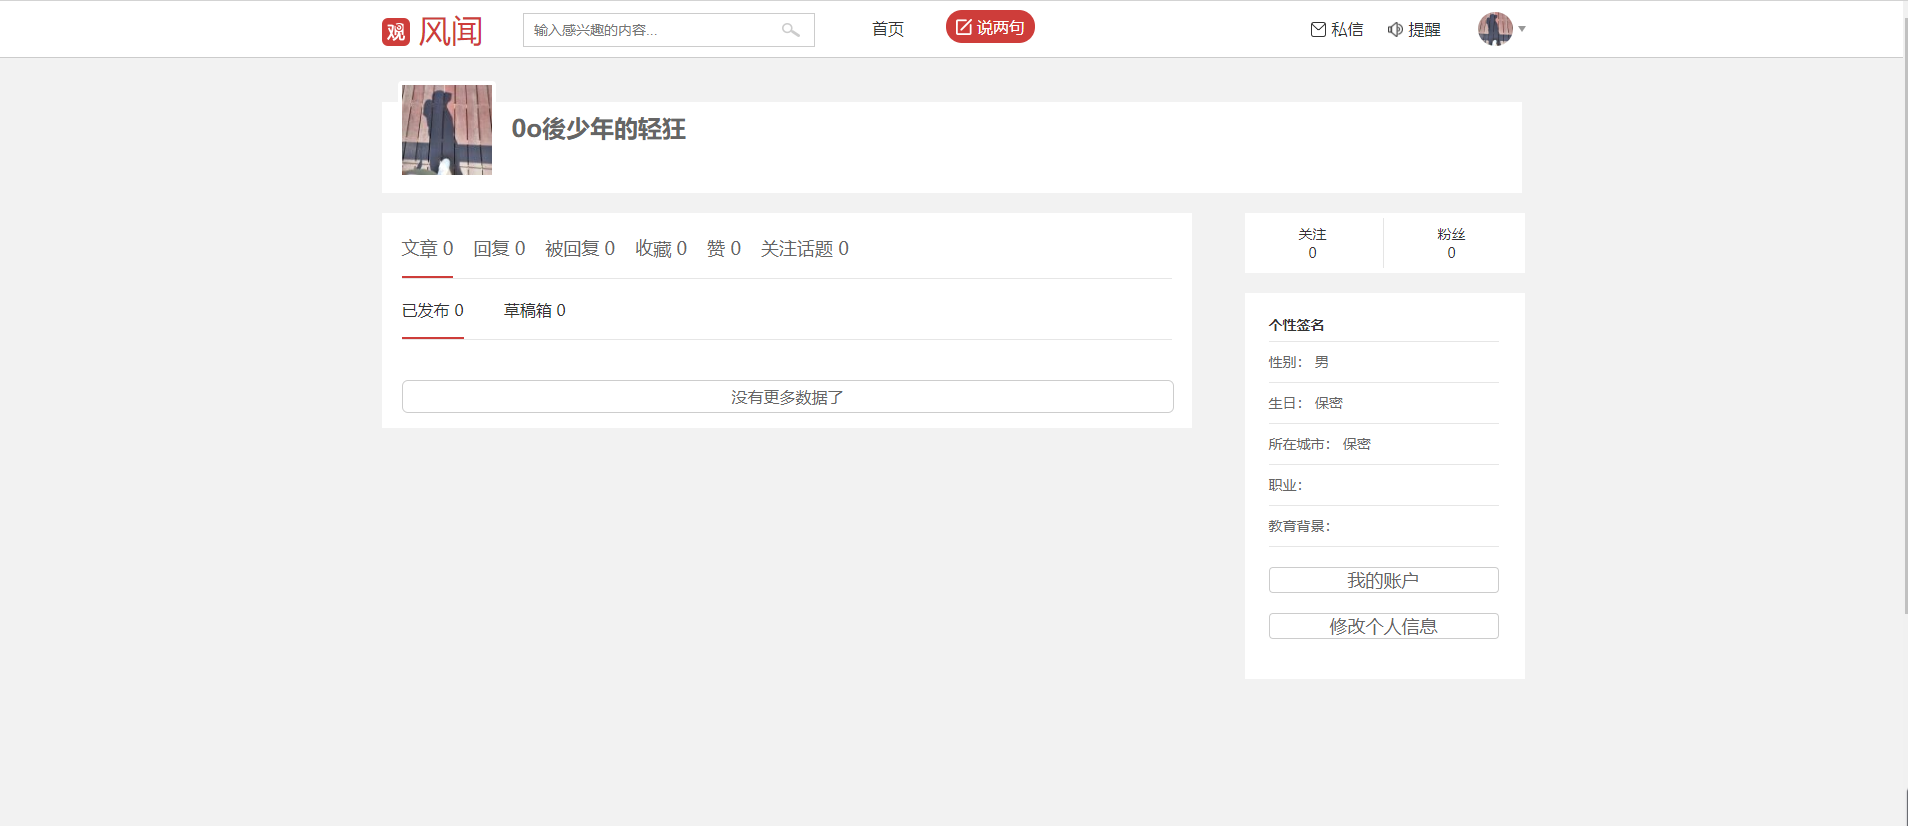
\includegraphics[scale=0.2]{观察者}
    	\caption{观察者}
    	\label{fig:github}
    \end{figure}



	\begin{figure}[h!]
		\centering
		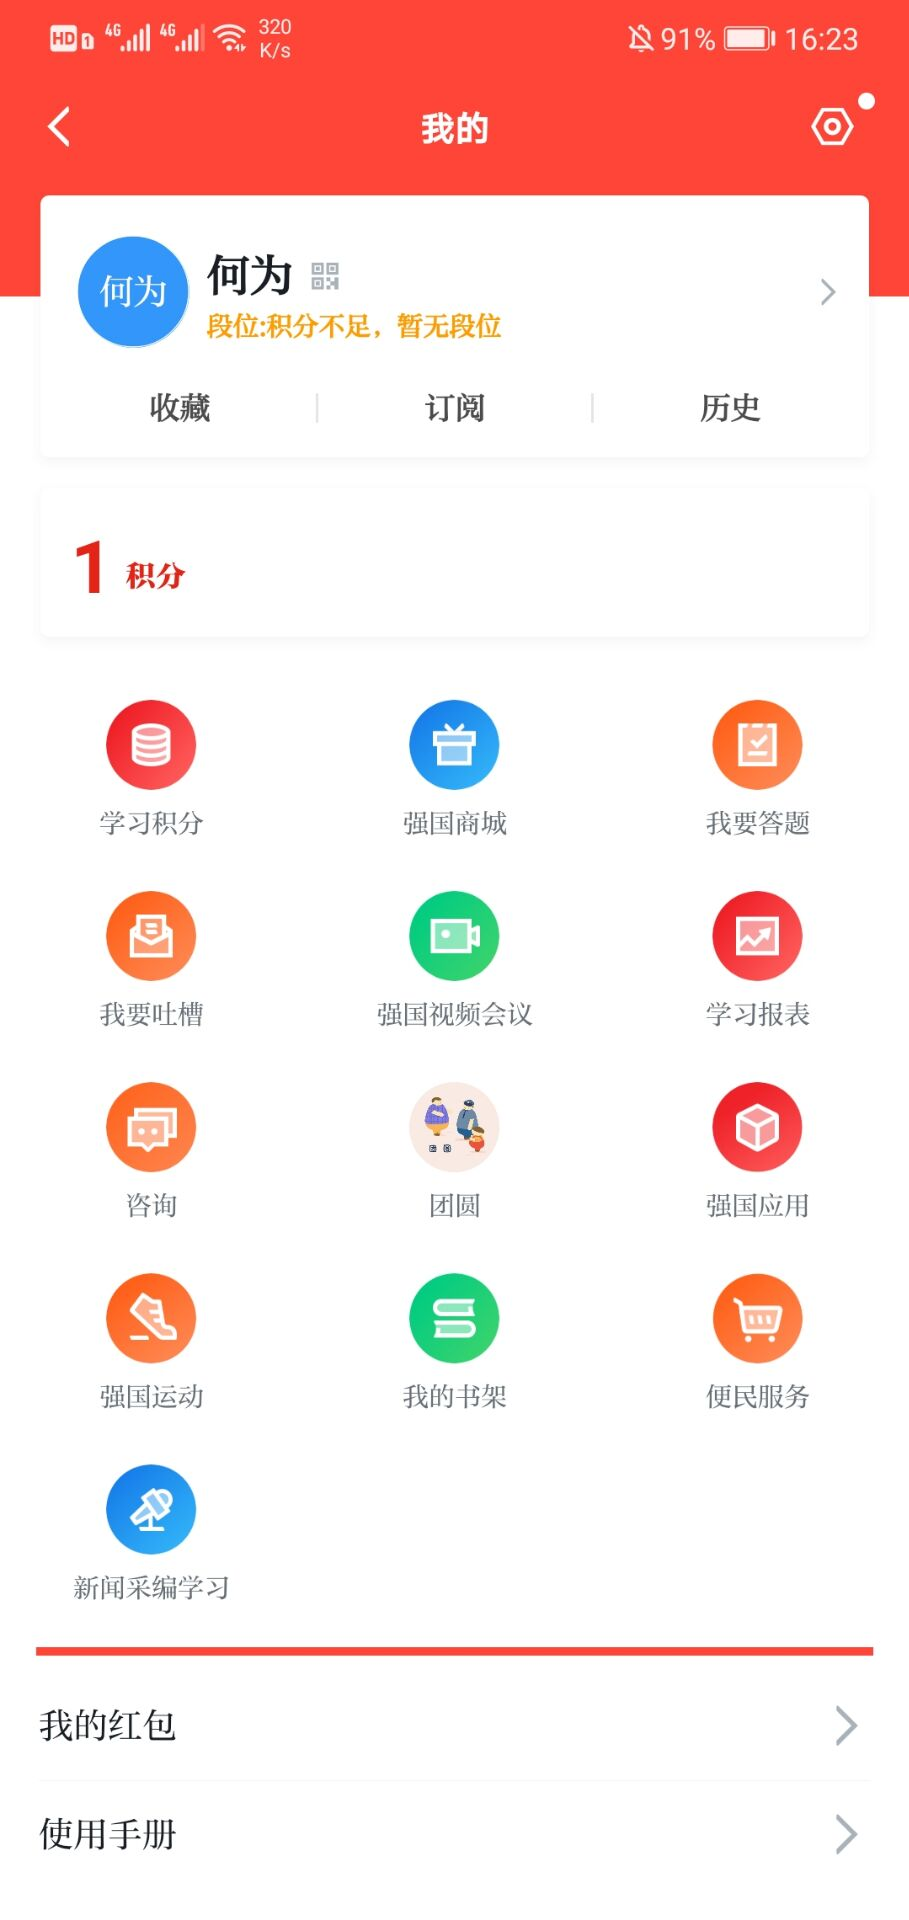
\includegraphics[scale=0.2]{学习强国}
		\caption{学习强国}
		\label{fig:github}
	\end{figure}



	\begin{figure}[h!]
	\centering
	
\includegraphics[scale=0.2]{b站}
	\caption{哔哩哔哩APP}
	\label{fig:github}
	\end{figure}

    \item 注册CSDN、博客园账户,给出个人网址和个人网站截图
    \begin{figure}[h!]
    	\centering
    	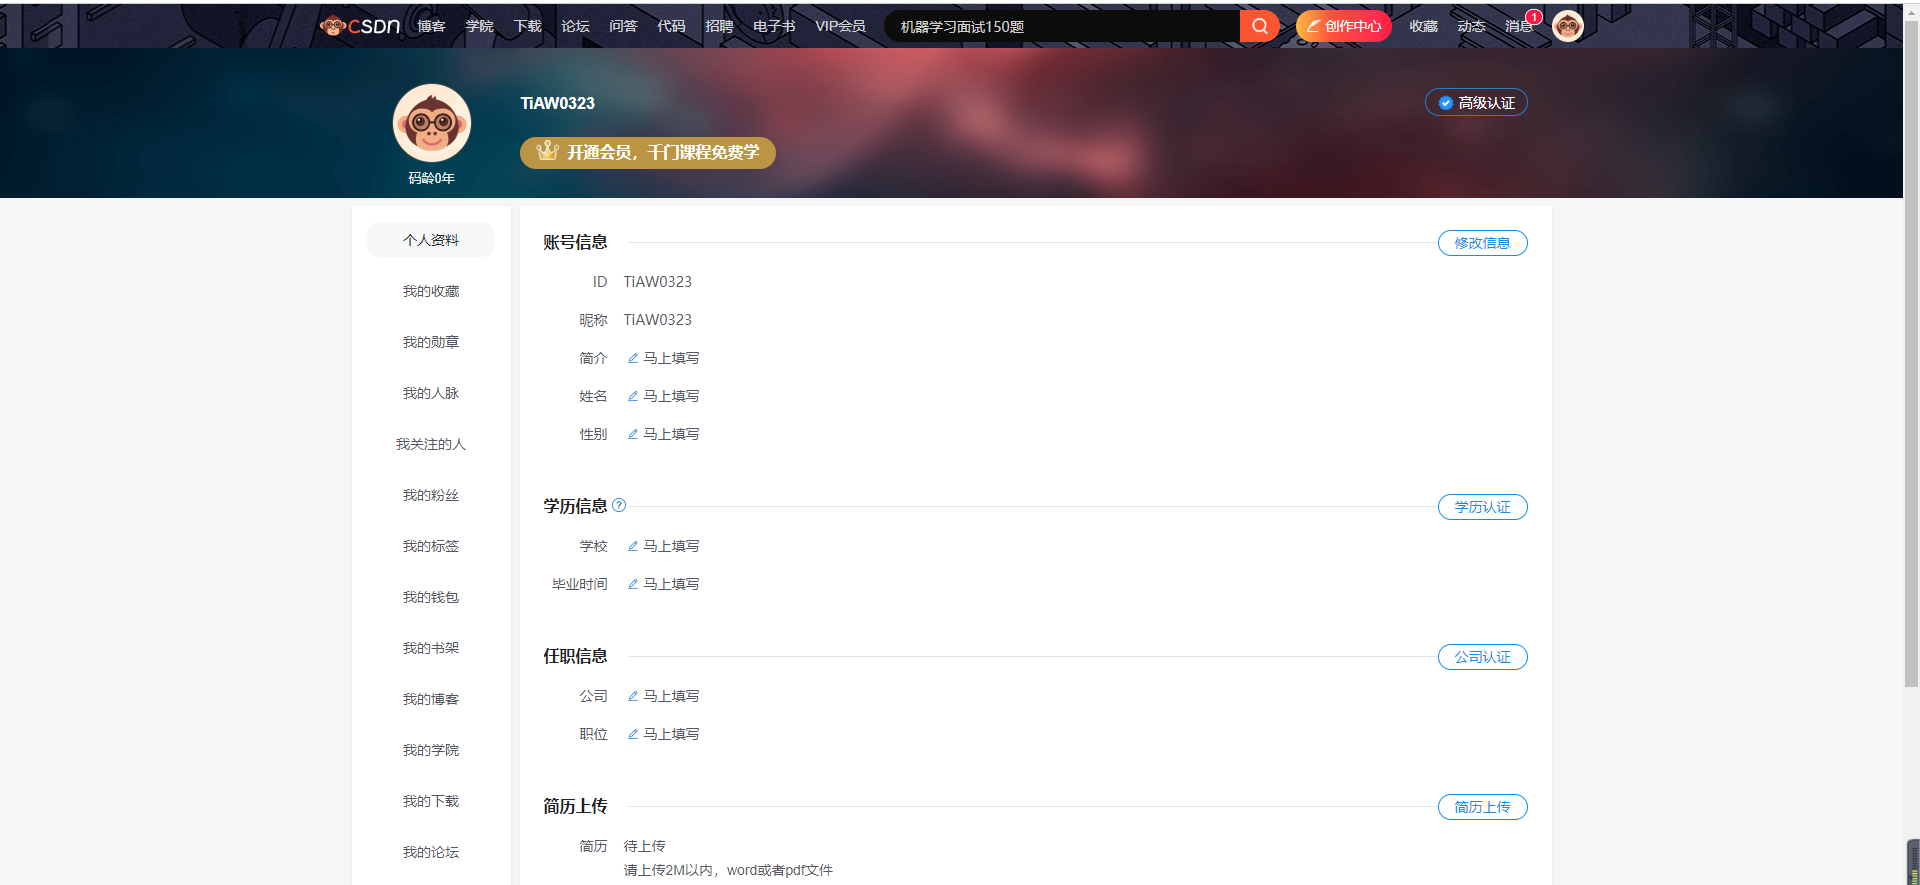
\includegraphics[scale=0.2]{CSDN}
    	\caption{CSDN网站:https://blog.csdn.net/TiAW0323?spm=1010.2135.3001.5113}
    	\label{fig:github}
    \end{figure}
\begin{figure}[h!]
	\centering
	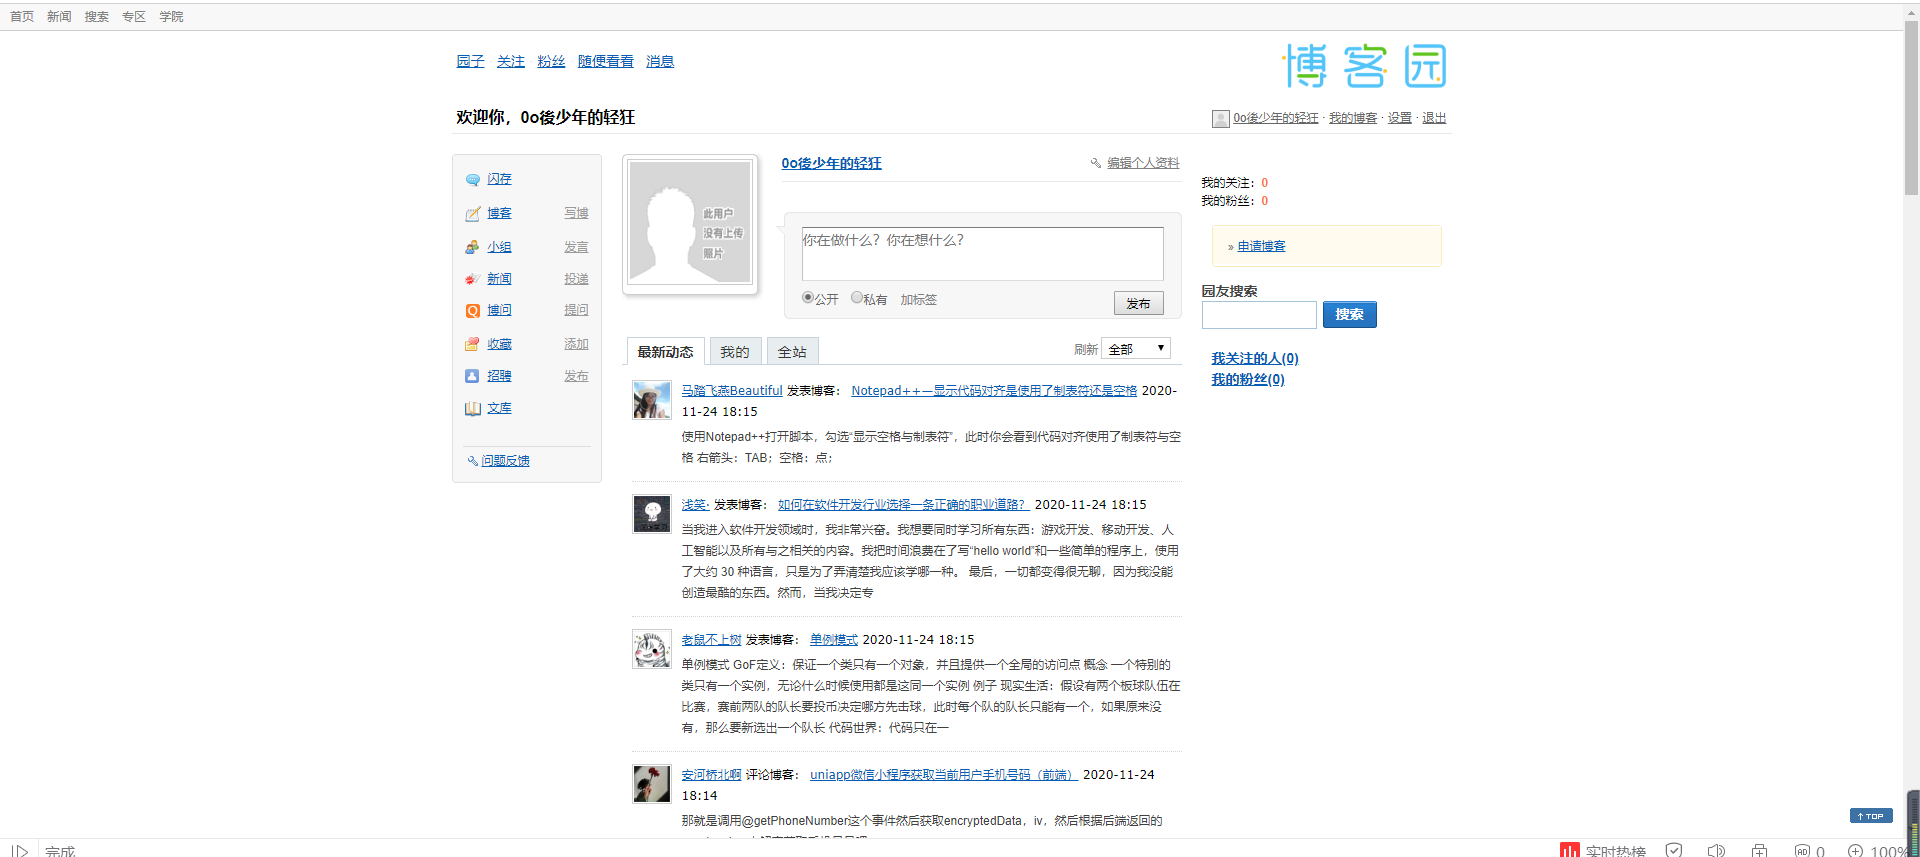
\includegraphics[scale=0.2]{博客园}
	\caption{博客园网站:https://home.cnblogs.com/ }
	\label{fig:github}
\end{figure}
    \item 注册小木虫账户,给出个人网址和个人网站截图
\end{itemize}
	\begin{figure}[h!]
		\centering
		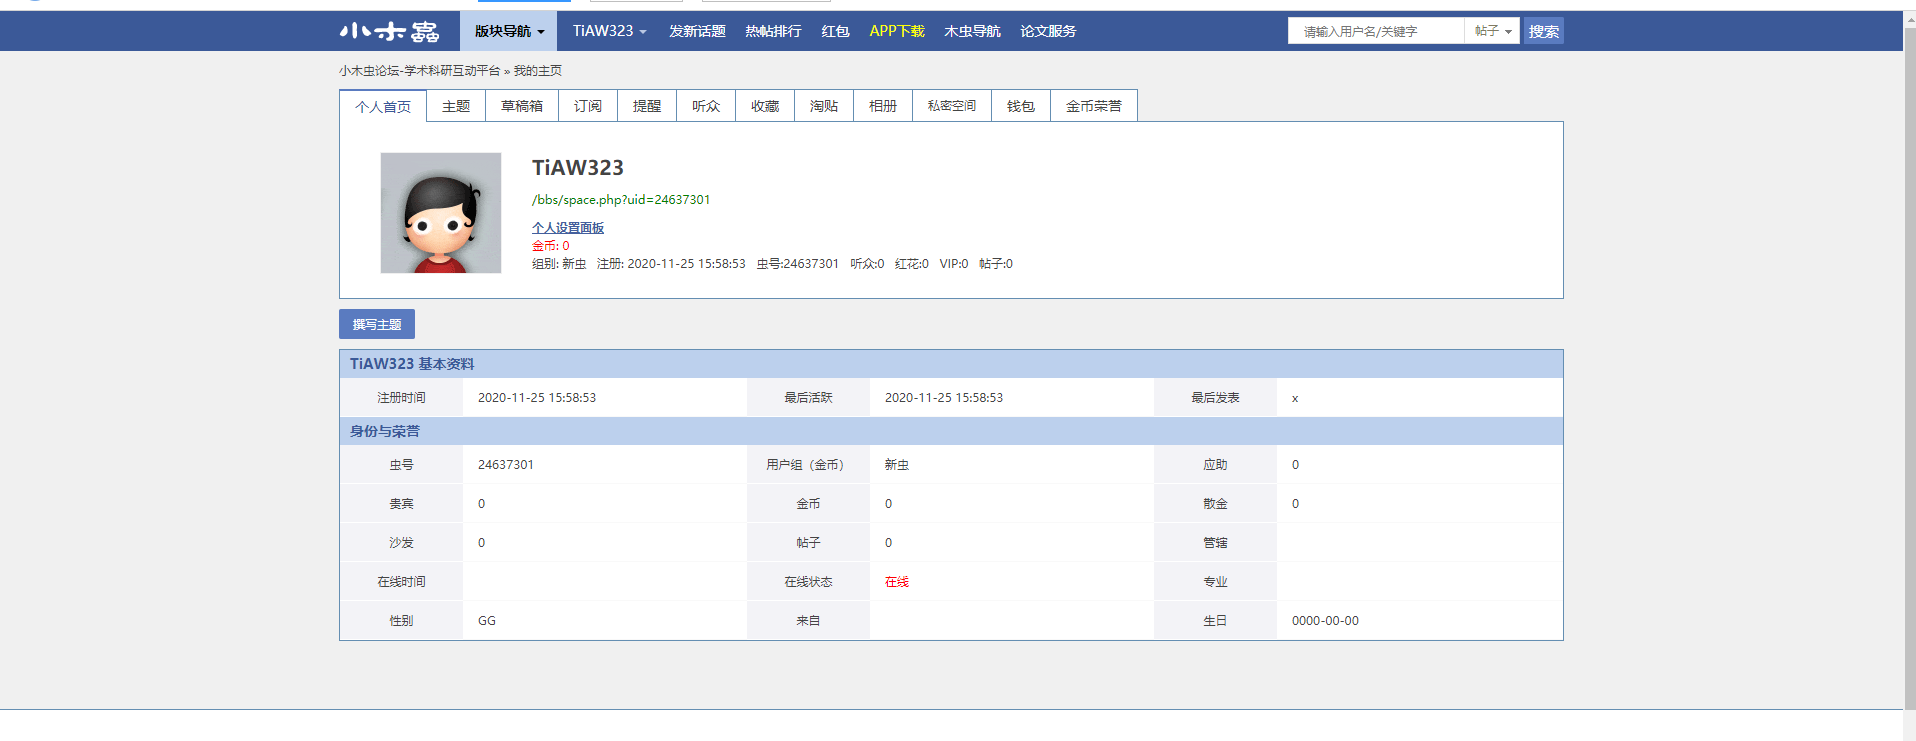
\includegraphics[scale=0.2]{小木虫}
		\caption{小木虫网址:http://muchong.com/bbs/space.php?uid=24637301}
		\label{fig:github}
	\end{figure}


\hspace*{\fill} \\

{\bf 注意,参考文献至少五篇,其中至少两篇为英文文献,参考文献必须在正文中有引用。}
\bibliographystyle{plain}
\bibliography{references}


\end{document}
